\documentclass{standalone}
\usepackage{tikz}
\usetikzlibrary{patterns, positioning}
\usepackage[sfdefault]{ClearSans} %% option 'sfdefault' activates Clear Sans as the default text font
\usepackage[T1]{fontenc}

\begin{document}
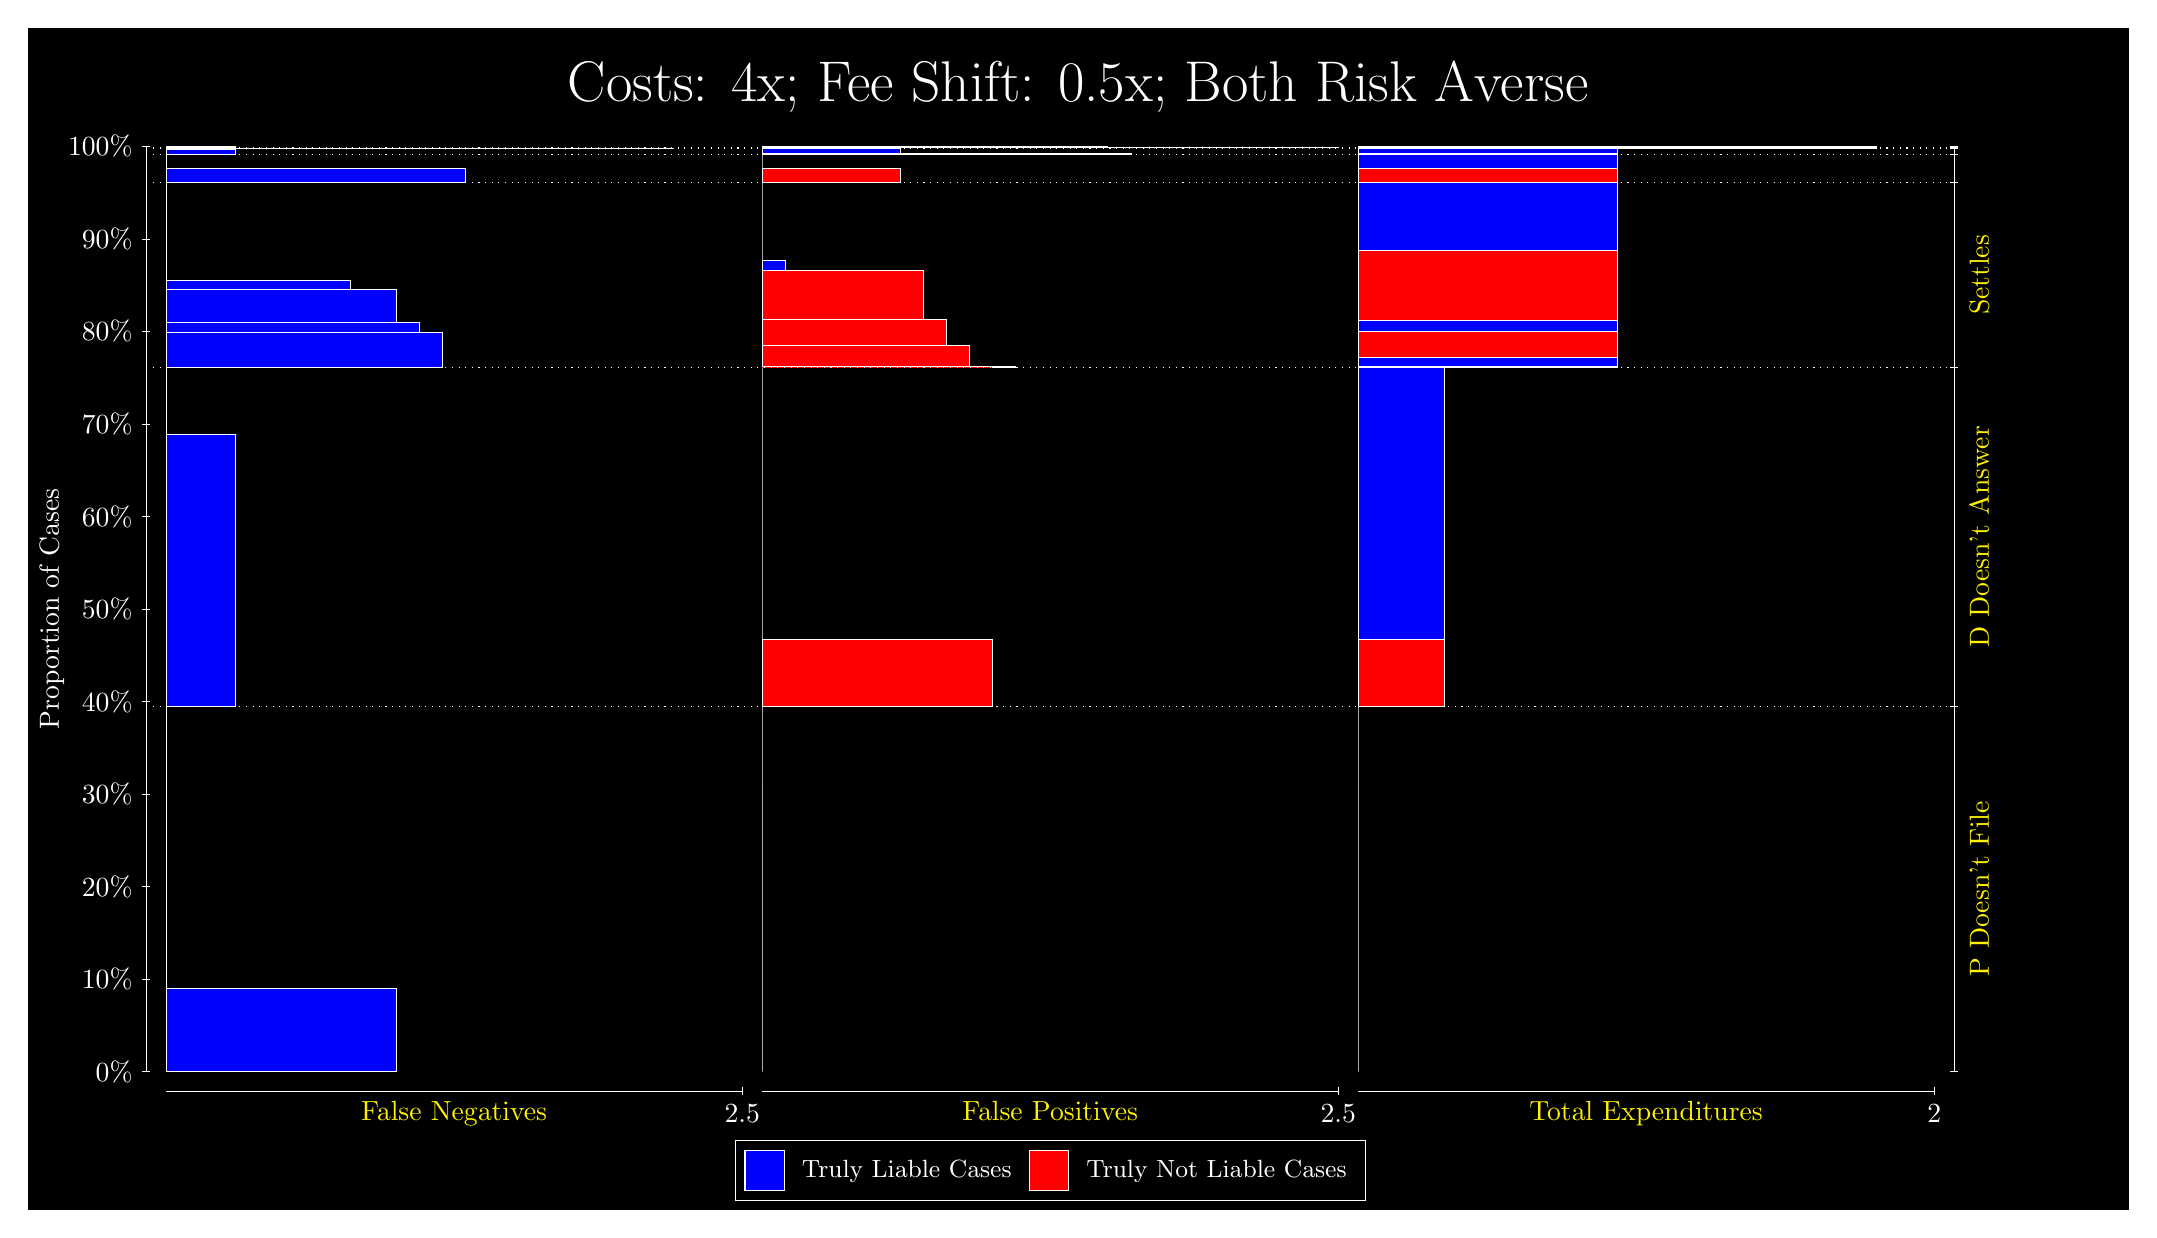
\begin{tikzpicture}
\draw[fill=black] (0,0) rectangle (26.667,15);
\draw[text=white] (0,13.5) rectangle (26.667,15) node[midway] {\huge Costs: 4x; Fee Shift: 0.5x; Both Risk Averse};
\draw[white, very thin] (1.5,1.75) -- (1.5,13.5);
\node[rotate=90, text=white, anchor=center] at (0.3, 7.625) {Proportion of Cases};
\draw[white, very thin] (1.45,1.75) -- (1.55,1.75);
\node[text=white, anchor=east] at (1.45, 1.75) {0\%};
\draw[white, very thin] (1.45,2.925) -- (1.55,2.925);
\node[text=white, anchor=east] at (1.45, 2.925) {10\%};
\draw[white, very thin] (1.45,4.1) -- (1.55,4.1);
\node[text=white, anchor=east] at (1.45, 4.1) {20\%};
\draw[white, very thin] (1.45,5.275) -- (1.55,5.275);
\node[text=white, anchor=east] at (1.45, 5.275) {30\%};
\draw[white, very thin] (1.45,6.45) -- (1.55,6.45);
\node[text=white, anchor=east] at (1.45, 6.45) {40\%};
\draw[white, very thin] (1.45,7.625) -- (1.55,7.625);
\node[text=white, anchor=east] at (1.45, 7.625) {50\%};
\draw[white, very thin] (1.45,8.8) -- (1.55,8.8);
\node[text=white, anchor=east] at (1.45, 8.8) {60\%};
\draw[white, very thin] (1.45,9.975) -- (1.55,9.975);
\node[text=white, anchor=east] at (1.45, 9.975) {70\%};
\draw[white, very thin] (1.45,11.15) -- (1.55,11.15);
\node[text=white, anchor=east] at (1.45, 11.15) {80\%};
\draw[white, very thin] (1.45,12.325) -- (1.55,12.325);
\node[text=white, anchor=east] at (1.45, 12.325) {90\%};
\draw[white, very thin] (1.45,13.5) -- (1.55,13.5);
\node[text=white, anchor=east] at (1.45, 13.5) {100\%};

\draw[white, very thin] (24.457,1.75) -- (24.457,13.5);
\draw[white, very thin] (24.407,1.75) -- (24.507,1.75);
\node[anchor=west] at (24.407, 1.75) {};
\draw[white, very thin] (24.407,6.3882) -- (24.507,6.3882);
\node[anchor=west] at (24.407, 6.3882) {};
\draw[white, very thin] (24.407,10.688) -- (24.507,10.688);
\node[anchor=west] at (24.407, 10.688) {};
\draw[white, very thin] (24.407,13.046) -- (24.507,13.046);
\node[anchor=west] at (24.407, 13.046) {};
\draw[white, very thin] (24.407,13.401) -- (24.507,13.401);
\node[anchor=west] at (24.407, 13.401) {};
\draw[white, very thin] (24.407,13.478) -- (24.507,13.478);
\node[anchor=west] at (24.407, 13.478) {};
\draw[white, very thin] (24.407,13.485) -- (24.507,13.485);
\node[anchor=west] at (24.407, 13.485) {};
\draw[white, very thin] (24.407,13.5) -- (24.507,13.5);
\node[anchor=west] at (24.407, 13.5) {};

\draw[white, very thin, fill=blue] (1.75,1.75) rectangle (4.6775,2.8028);
\draw[white, very thin, fill=red] (1.75,2.8028) rectangle (1.75,6.3882);
\draw[white, very thin, fill=blue] (1.75,6.3882) rectangle (2.6283,9.8389);
\draw[white, very thin, fill=red] (1.75,9.8389) rectangle (1.75,10.688);
\draw[white, very thin, fill=blue] (1.75,10.688) rectangle (5.2631,11.136);
\draw[white, very thin, fill=blue] (1.75,11.136) rectangle (4.9703,11.269);
\draw[white, very thin, fill=blue] (1.75,11.269) rectangle (4.6775,11.681);
\draw[white, very thin, fill=blue] (1.75,11.681) rectangle (4.3848,11.683);
\draw[white, very thin, fill=blue] (1.75,11.683) rectangle (4.092,11.805);
\draw[white, very thin, fill=red] (1.75,11.805) rectangle (1.75,13.046);
\draw[white, very thin, fill=blue] (1.75,13.046) rectangle (5.5558,13.225);
\draw[white, very thin, fill=red] (1.75,13.225) rectangle (1.75,13.401);
\draw[white, very thin, fill=blue] (1.75,13.401) rectangle (2.6283,13.461);
\draw[white, very thin, fill=red] (1.75,13.461) rectangle (1.75,13.478);
\draw[white, very thin, fill=blue] (1.75,13.478) rectangle (8.1906,13.481);
\draw[white, very thin, fill=red] (1.75,13.481) rectangle (1.75,13.485);
\draw[white, very thin, fill=blue] (1.75,13.485) rectangle (2.6283,13.497);
\draw[white, very thin, fill=red] (1.75,13.497) rectangle (1.75,13.5);
\draw[white, very thin, fill=red] (9.3189,1.75) rectangle (9.3189,5.3354);
\draw[white, very thin, fill=blue] (9.3189,5.3354) rectangle (9.3189,6.3882);
\draw[white, very thin, fill=red] (9.3189,6.3882) rectangle (12.246,7.2373);
\draw[white, very thin, fill=blue] (9.3189,7.2373) rectangle (9.3189,10.688);
\draw[white, very thin, fill=red] (9.3189,10.688) rectangle (12.539,10.702);
\draw[white, very thin, fill=red] (9.3189,10.702) rectangle (12.246,10.703);
\draw[white, very thin, fill=red] (9.3189,10.703) rectangle (11.954,10.969);
\draw[white, very thin, fill=red] (9.3189,10.969) rectangle (11.661,11.299);
\draw[white, very thin, fill=red] (9.3189,11.299) rectangle (11.368,11.929);
\draw[white, very thin, fill=blue] (9.3189,11.929) rectangle (9.6116,12.05);
\draw[white, very thin, fill=blue] (9.3189,12.05) rectangle (9.3189,13.046);
\draw[white, very thin, fill=red] (9.3189,13.046) rectangle (11.075,13.222);
\draw[white, very thin, fill=blue] (9.3189,13.222) rectangle (9.3189,13.401);
\draw[white, very thin, fill=red] (9.3189,13.401) rectangle (14.003,13.418);
\draw[white, very thin, fill=blue] (9.3189,13.418) rectangle (11.075,13.478);
\draw[white, very thin, fill=red] (9.3189,13.478) rectangle (11.075,13.481);
\draw[white, very thin, fill=blue] (9.3189,13.481) rectangle (9.3189,13.485);
\draw[white, very thin, fill=red] (9.3189,13.485) rectangle (16.638,13.488);
\draw[white, very thin, fill=blue] (9.3189,13.488) rectangle (13.71,13.5);
\draw[white, very thin, fill=red] (16.888,1.75) rectangle (16.888,5.3354);
\draw[white, very thin, fill=blue] (16.888,5.3354) rectangle (16.888,6.3882);
\draw[white, very thin, fill=red] (16.888,6.3882) rectangle (17.986,7.2373);
\draw[white, very thin, fill=blue] (16.888,7.2373) rectangle (17.986,10.688);
\draw[white, very thin, fill=red] (16.888,10.688) rectangle (20.181,10.702);
\draw[white, very thin, fill=blue] (16.888,10.702) rectangle (20.181,10.824);
\draw[white, very thin, fill=red] (16.888,10.824) rectangle (20.181,11.154);
\draw[white, very thin, fill=blue] (16.888,11.154) rectangle (20.181,11.287);
\draw[white, very thin, fill=red] (16.888,11.287) rectangle (20.181,12.184);
\draw[white, very thin, fill=blue] (16.888,12.184) rectangle (20.181,13.046);
\draw[white, very thin, fill=red] (16.888,13.046) rectangle (20.181,13.222);
\draw[white, very thin, fill=blue] (16.888,13.222) rectangle (20.181,13.401);
\draw[white, very thin, fill=red] (16.888,13.401) rectangle (20.181,13.418);
\draw[white, very thin, fill=blue] (16.888,13.418) rectangle (20.181,13.478);
\draw[white, very thin, fill=red] (16.888,13.478) rectangle (23.475,13.481);
\draw[white, very thin, fill=blue] (16.888,13.481) rectangle (23.475,13.485);
\draw[white, very thin, fill=red] (16.888,13.485) rectangle (23.475,13.488);
\draw[white, very thin, fill=blue] (16.888,13.488) rectangle (23.475,13.5);
\draw[white, dotted] (1.5,6.3882) -- (24.457,6.3882);
\draw[white, dotted] (1.5,10.688) -- (24.457,10.688);
\draw[white, dotted] (1.5,13.046) -- (24.457,13.046);
\draw[white, dotted] (1.5,13.401) -- (24.457,13.401);
\draw[white, dotted] (1.5,13.478) -- (24.457,13.478);
\draw[white, dotted] (1.5,13.485) -- (24.457,13.485);
\draw[white, very thin] (1.75,1.5) -- (9.0689,1.5);
\node[text=yellow, anchor=north] at (5.4094, 1.5) {False Negatives};
\draw[white, very thin] (9.0689,1.45) -- (9.0689,1.55);
\node[text=white, anchor=north] at (9.0689, 1.45) {2.5};

\draw[white, very thin] (9.3189,1.5) -- (16.638,1.5);
\node[text=yellow, anchor=north] at (12.978, 1.5) {False Positives};
\draw[white, very thin] (16.638,1.45) -- (16.638,1.55);
\node[text=white, anchor=north] at (16.638, 1.45) {2.5};

\draw[white, very thin] (16.888,1.5) -- (24.207,1.5);
\node[text=yellow, anchor=north] at (20.547, 1.5) {Total Expenditures};
\draw[white, very thin] (24.207,1.45) -- (24.207,1.55);
\node[text=white, anchor=north] at (24.207, 1.45) {2};

\node[text=yellow, centered, rotate=90] at (24.777, 4.0691) {P Doesn't File};
\node[text=yellow, centered, rotate=90] at (24.777, 8.5381) {D Doesn't Answer};
\node[text=yellow, centered, rotate=90] at (24.777, 11.867) {Settles};





\draw (12.978300999999998,1.5) node[draw=none] (baseCoordinate) {};
\begin{scope}[align=center]
        \matrix[scale=0.5, draw=white, below=0.5cm of baseCoordinate, nodes={draw}, column sep=0.1cm]{
            \node[rectangle, draw, minimum width=0.5cm, minimum height=0.5cm, fill=blue] {}; &
            \node[draw=none, font=\small, text=white] (B) {Truly Liable Cases}; &
            \node[rectangle, draw, minimum width=0.5cm, minimum height=0.5cm, fill=red] {}; &
            \node[draw=none, font=\small, text=white] (B) {Truly Not Liable Cases}; \\
            };
\end{scope}

\end{tikzpicture}
\end{document}